\documentclass{article}
\usepackage{biblatex} %Imports biblatex package
\addbibresource{refs.bib} %Import the bibliography file
\usepackage[utf8]{inputenc}

\usepackage[top=1in, bottom=1in, left=1in, right=1in]{geometry}

\usepackage[onehalfspacing]{setspace}

\usepackage{amsmath, amssymb, amsthm}
\usepackage{enumerate, enumitem}
\usepackage{fancyhdr, graphicx, proof, comment, multicol}
\usepackage[none]{hyphenat}
\usepackage{dirtytalk}
\binoppenalty=\maxdimen
\relpenalty=\maxdimen
\usepackage{microtype}
%\usepackage{mathpazo}
\usepackage{mdframed}
\usepackage{parskip}
\linespread{1.1}
\usepackage{graphicx}
\usepackage{subfig}
\usepackage{mathrsfs}
\usepackage{amsfonts}
\usepackage{amsmath}
\usepackage{minted}
\usepackage{amssymb}
\usepackage{algorithm}
\usepackage[noend]{algpseudocode}
\usepackage{mathtools}
\usepackage{hyperref}


\title{Operating system \LaTeX template}
\author{Rubén Ballester Bautista}
\date{December 2021}

%%%%%%%%%%%%%%%%%%%%%%%%%%%%%%%%%%%%%%%%%%%%%%%%%%%%%%%%%%%%%%%%%%%%%%%%%
% theorem environments
%%%%%%%%%%%%%%%%%%%%%%%%%%%%%%%%%%%%%%%%%%%%%%%%%%%%%%%%%%%%%%%%%%%%%%%%%

\newtheorem{defn0}{Definition}[section]
\newtheorem{prop0}[defn0]{Proposition}
\newtheorem{thm0}[defn0]{Theorem}
\newtheorem{lemma0}[defn0]{Lemma}
\newtheorem{corollary0}[defn0]{Corollary}
\newtheorem{example0}[defn0]{Example}
\newtheorem{remark0}[defn0]{Remark}
\newtheorem{conjecture0}[defn0]{Conjecture}

\newenvironment{definition}{ \begin{defn0}}{\end{defn0}}
\newenvironment{proposition}{\bigskip \begin{prop0}}{\end{prop0}}
\newenvironment{theorem}{\bigskip \begin{thm0}}{\end{thm0}}
\newenvironment{lemma}{\bigskip \begin{lemma0}}{\end{lemma0}}
\newenvironment{corollary}{\bigskip \begin{corollary0}}{\end{corollary0}}
\newenvironment{example}{ \begin{example0}\rm}{\end{example0}}
\newenvironment{remark}{ \begin{remark0}\rm}{\end{remark0}}
\newenvironment{conjecture}{\begin{conjecture0}}{\end{conjecture0}}

\newcommand{\defref}[1]{Definition~\ref{#1}}
\newcommand{\propref}[1]{Proposition~\ref{#1}}
\newcommand{\thmref}[1]{Theorem~\ref{#1}}
\newcommand{\lemref}[1]{Lemma~\ref{#1}}
\newcommand{\cororef}[1]{Corollary~\ref{#1}}
\newcommand{\exref}[1]{Example~\ref{#1}}
\newcommand{\secref}[1]{Section~\ref{#1}}
\newcommand{\remref}[1]{Remark~\ref{#1}}
\newcommand{\conjref}[1]{Conjecture~\ref{#1}}
\DeclarePairedDelimiterX{\norm}[1]{\lVert}{\rVert}{#1}

\begin{document}

\maketitle

\begin{center}
    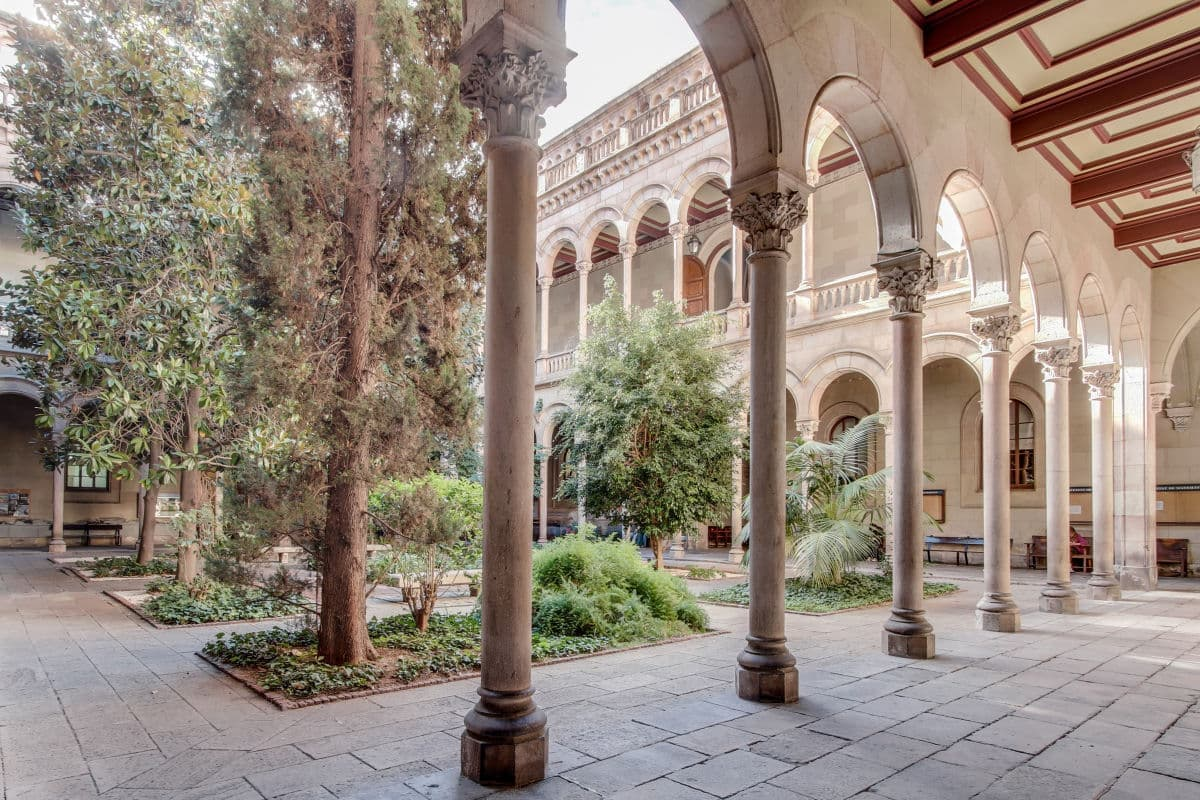
\includegraphics[width=0.9\textwidth]{images/example.jpg}
\end{center}

\section{Abstract (summary)}

Here you should summarise what you did in the lab.

\section{Experiments and results}
\subsection{Exercise 1}
Here you should put all your tests to check the correct behaviour of your code.
\subsection{Exercise 2}
Bla bla bla...
\section{Conclusions}

\begin{equation}
    P: (-2\alpha)x + (-2\beta)y + z = r^2 - (\alpha^2 + \beta^2).
\end{equation}

\section{Algorithms}
\begin{algorithm}
\begin{algorithmic}[1]
\Procedure{FindEnclosingDisk}{$A,B$}
    \State $A^*,B^*\leftarrow$liftToParaboloid($A,B$)
    \State \texttt{satisfied}, $D$ $\leftarrow MegiddoAlgorithm(A^*,B^*$) 
    \State if \texttt{satisfied} then \Return $D$, else \Return False
\EndProcedure
\end{algorithmic}
\end{algorithm}
\subsection{Bash code}
\begin{minted}{bash}
#!/bin/bash
echo "Enter directory name"
read ndir
if [ -d "$ndir" ]
then
echo "Directory exist"
else
`mkdir $ndir`
echo "Directory created"
fi
\end{minted}
You can put references  using the cite command \cite{linearProg}.

% BIBLIOGRAPHY (References)

\printbibliography
\end{document}